\chapter{ESTADO DEL ARTE}

\section{Rob\'otica en Miner\'ia}
La minería actual ha llevado a que las compañías mineras busquen la eficiencia 
incorporando la robótica a sus procesos, generando, adicionalmente, una fuente 
fructífera de innovación local. Actualmente el país sudamericano con mayor inversión 
en minería es el país de Chile, este país ha iniciado la robótica en su país hace 
unos 15 años \cite{Carmona2014}.

Los beneficios potenciales de los robots en la minería subterránea son abundantes. Debido 
a que estas zonas son entornos de trabajo extenuante y potencialmente peligroso para 
los seres humanos. Por tal motivo, dándole un mayor grado de autonomía a los robots, estos 
se convierten en buenos ayudantes para los mineros o incluso pueden sustituir el personal 
que se despliega en los socavones \cite{Carmona2014}. Hace 20 años se empezó a realizar 
investigaciones sobre autonomía en la minería subterránea utilizando una máquina de carga 
con sensores láser y de ultrasonido que transportaba los minerales por las minas 
subterráneas \cite{Scheding1999}. 

Este trabajo  de investigación  se enfoca en la inspección de socavones subterráneos, por 
ende en el año 2003 “\textit{Groundhog}” fue el primer robot que exploró la mina de 
Florencia (\textit{New Eagle}) \cite{Thrun2004}, empleando sensores láser y una cámara de 
video. Asimismo en Alemania se creó un robot móvil llamado “\textit{Alexander}” el cual 
exploró la mina de oro \textit{Reiche Zeche} en Freiberg \cite{Grehl2015}.

Para la generación de los modelos geométricos visuales en 3D como primer trabajo en el 
año 2014 se utilizó una camioneta equipada de sensores láser y un microprocesador, los 
cuales ayudaron a realización de un modelo en 3D de la mina \cite{Zlot2014}. Como trabajo 
a futuro de esta investigación, es pasar el software, para obtener el modelo visual 3D, 
a un robot móvil.
 
El robot utilizará la técnica SLAM para su desplazamiento. Anteriores trabajos 
respaldan en que este método es la más adecuada para la autonomía del robot, así como es 
en el caso del robot móvil minero “\textit{QHUBOT}” , que utiliza la técnica FastSLAM para 
poder desplazarse sobre los socavones subterráneos \cite{Mauricio2015}, así también 
en \cite{Thrun2004} utilizan la técnica de SLAM para la exploración de la mina abandona. 

Actualmente, hay trabajos de investigación en los que estudian drones con el algoritmo SLAM 
donde unos se orientan a resolver problemas de navegación utilizando algoritmos de seguimiento 
de líneas basados en la visión \cite{Verschoor2013}. El algoritmo basado en la visión se 
emplea en las diversas estructuras lineales, que reflejan el entorno construido por los 
seres humanos, donde se implementa un algoritmo SLAM acompañado de los puntos que detecta 
una cámara. Así la misma lógica del uso de SLAM se refleja en el paper \cite{Skoda2015} 
solo que los autores describen el uso de drones en la situación muy especializado como lo 
son de rescate. El objetivo es enviar el drone para que genere un mapa 3D antes de enviar 
al personal de emergencias. El mapa es generado por la costura de varias imágenes de una 
cámara RGBD (\textit{RGB y profundidad de imagen}). Algo similar se puede ver en el 
paper \cite{Heukels2015} el cual el algoritmo SLAM se utiliza después de realizar 
procesamiento de imágenes a las imágenes obtenidas de una cámara.

Comercialmente existe drones que cumplen la función buscada (\textit{generar mapas}), como 
es el caso de la empresa Canadiense llamada \textit{Clickmox Solutions}, que ha 
desarrollado un drone llamado “\textit{MineFly Drone}”, el cual tiene un escáner 
láser que genera mapas en las minas subterráneas. El drone está integrado con una 
luz LED, sensores sonar, una cámara HD y emplea la técnica de SLAM para poder 
desplazarse por todo el socavón sin la necesidad de utilizar un GPS \cite{Solutions2016}. 


\section{Control de Robots M\'oviles}
\begin{figure}%[ht!]
  \centering \footnotesize
  %\subfloat[Attractive Force]{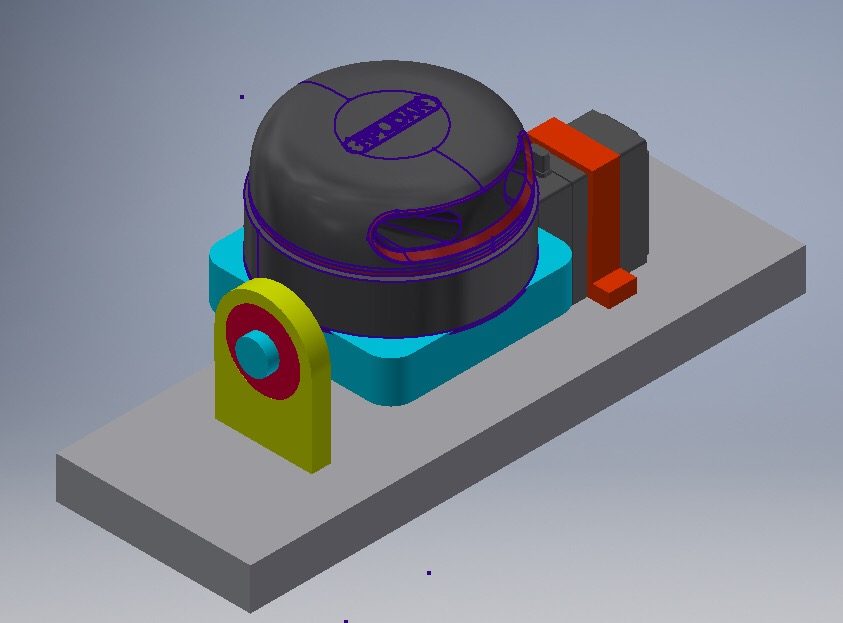
\includegraphics[width=0.16\textwidth]{images/lidar_3D.jpeg}}
  %~\subfloat[Repulsive Force]{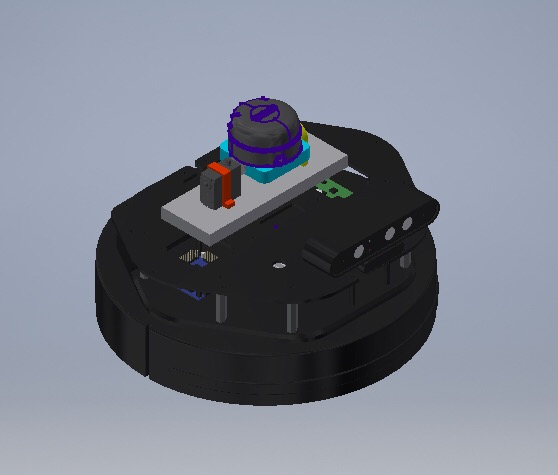
\includegraphics[width=0.16\textwidth]{images/kbki_lidar3D.jpeg}} 
  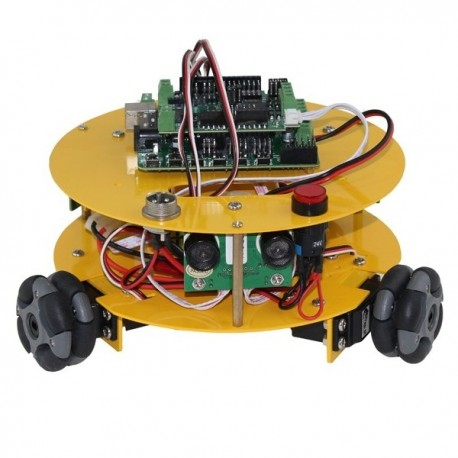
\includegraphics[width=0.35\textwidth]{images/omnidirecional.jpg}
  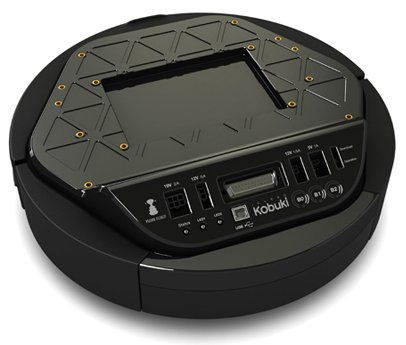
\includegraphics[width=0.35\textwidth]{images/kobuki.jpg}
  \\ $\qquad\qquad$ a. Sistema mecánico $\qquad\qquad$  b. Implementado en el Kobuki
  %\subfloat[Navigation Force]{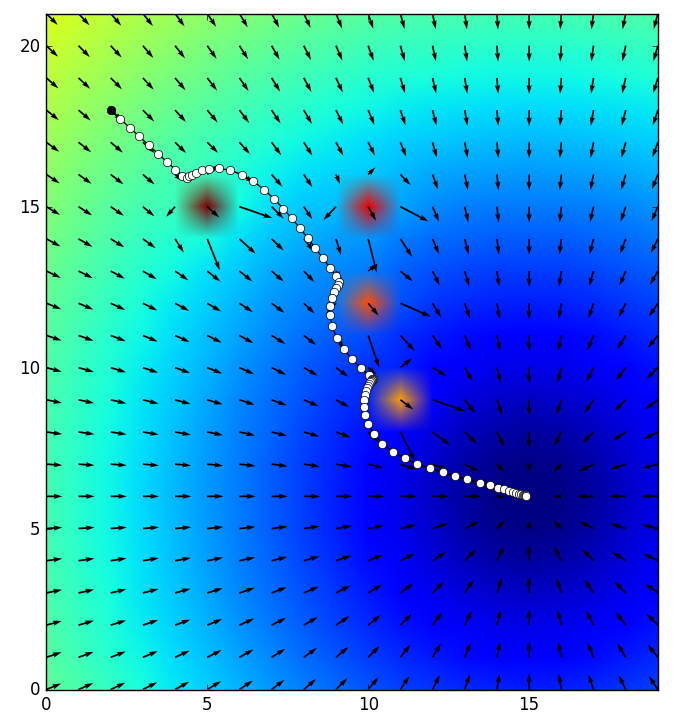
\includegraphics[width=0.16\textwidth]{images/nav_force.png}}
  % \subfloat[Attractive Force]{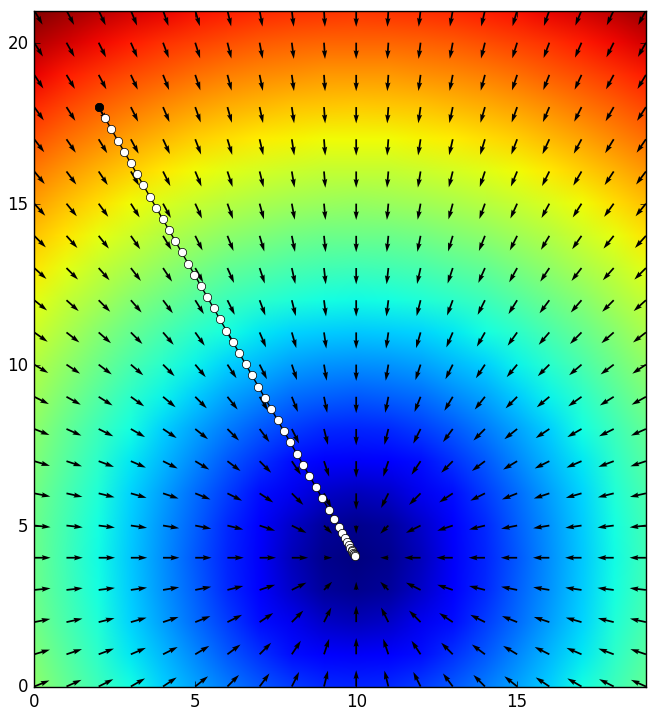
\includegraphics[width = 150mm]{attr_force.png}}
  \captionsetup{font=footnotesize}
  \caption{Tests for the Potential Field Algorithm: (right) Sistema mecánico, (left) Implementado en el Kobuki} 
  \label{f:omnidirectional}
\end{figure}
La generaci\'on de movimiento del robot m\'ovil necesita de un control cinem\'atico 
adecuado. El objetivo de un controlador cinem\'atico es seguir una trayectoria descrita 
por su posici\'on o perfil de velocidad como una funci\'on del tiempo. Esto se hace 
a menudo dividiendo la trayectoria en segmentos de movimiento de forma claramente 
definida, por ejemplo, l\'ineas rectas y segmentos de un c\'irculo.

Un enfoque m\'as apropiado en el control de movimiento de un robot m\'ovil es usar 
un controlador de realimentaci\'on de estado real. Con un controlador de este tipo, 
la tarea de planificaci\'on de ruta del robot se reduce a establecer posiciones 
intermedias situadas en la ruta solicitada. Con este fin, primero debe calcularse 
el modelo cinem\'atico que relaciona la velocidad de las ruedas con la velocidad 
lineal y angular del robot en su propio marco de referencia. Luego utilizar las 
leyes de control que permite un suave movimiento en la trayectoria del robot. Esta 
secci\'on explica los controladores utilizados en los robots m\'oviles.

Para el control de movimiento de los robots móviles, se debe tener en consideración 
la clasificación de estos a través de la locomoción de sus ruedas. Esto se divide 
en dos: (1) robot holon\'omico y (2) robot no-holon\'omico. El robot holon\'omico 
no tiene ninguna restricci\'on, con respecto a la velocidad, en la posici\'on y 
la orientaci\'on. El robot se puede mover instant\'aneamente en cualquier direcci\'on 
del espacio, sin necesidad de rotar previamente. La mayor\'ia de estos robots 
m\'oviles son omnidireccionales, como se puede ver en la figura 
\ref{f:omnidirectional}. En cambio un robot no-holonomico tiene una restricci\'on 
en su velocidad, no existe un trayectoria que dependa solamente de la posici\'on y 
orientaci\'on. Por ende, este robot no se puede mover instant\'aneamente en cada 
direcci\'on del espacio. 

\subsection{Control Cinem\'atico PID}

Un controlador PID (Proporcional, Integral, Derivativa) es un mecanismo de control 
por realimentaci\'on. Este calcula la desviaci\'on o error entre un valor medido y 
un valor deseado. Este algoritmo de control consta de tres par\'ametros distintos: el 
proporcional, el integral y el derivativo. El valor proporcional depende del error 
actual. El integral depende de los errores pasados y el derivativo es una predicci\'on 
de los errores futuros. La suma de estas tres acciones es usada para ajustar al 
proceso por medio de un elemento de control. Este algoritmo es ampliamente 
difundido en el mundo industrial, cuya forma m\'as conocida es:
\begin{align*}
%\label{eqn:pid}
u(t) = K_c e(t) + \frac{K_c}{T_i} \int e(t)dt + K_c T_d \frac{de(t)}{dt} = P(t) + I(t) + D(t)
\end{align*}
donde $K_c$ es la ganancia proporcional, $T_i$ es el tiempo integral, $T_d$ es 
el tiempo derivativo y $e(t)$ es el error entre la posici\'on actual y la posici\'on deseada
del robot. Este algoritmo posee muchas variaciones, dependiendo de la aplicaci\'on el controlador 
en cuesti\'on puede trabajar como P, PI, PD o PID.

\subsection{Control Cinem\'atico Polar}

\begin{figure}%[h]
\centering \footnotesize
 {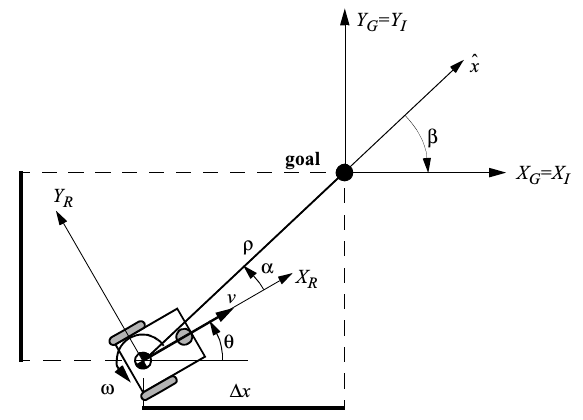
\includegraphics[width=0.60\linewidth]{images/control_polar.png}}
 \captionsetup{font=footnotesize}
 \caption{Configuraci\'on para el control polar donde se muestran la posici\'on del 
 objetivo y los par\'ametros espec\'ificos \cite{siegwart2011introduction}.}
\label{f:controlPolar}
\end{figure}

Una forma alternativa de obtener un control suave de posici\'on y orientaci\'on 
para un robot es a trav\'es de una ley lineal de control por realimentaci\'on 
de estados basada en coordenadas polares. Como muestra la Figura ~\ref{f:controlPolar}, 
las coordenadas polares asociadas con el robot son:
\begin{align*}
\rho &= \sqrt[]{(x_{d} - x)^2 + (y_{d} - y)^2} \\
\alpha &= \text{atan2}(y_{d} - y, x_{d} - x) - \theta \\
\beta &= -\text{atan2}(y_{d} - y, x_{d} - x) + \theta_{d}
\end{align*}
donde $\rho$ representa la distancia desde el robot a la posici\'on de la 
meta, $\alpha$ y $\beta$ son \'angulos que se utilizan para el error de 
orientaci\'on. La pose actual del robot es $\x=(x,y,\theta)$, y su pose 
deseada es $(x_{d},y_{d},\theta_{d})$. En base a estas variables polares, la 
ley de control que define las velocidades lineales y angulares para lograr 
la pose deseada es 
\begin{align}
\label{eqn:v}
v &= k_{\rho}\rho \\
\label{eqn:w}
\omega &= k_{\alpha}\alpha + k_{\beta}\beta
\end{align}
donde $k_{\rho}$, $k_{\alpha}$ y $k_{\beta}$ son las ganancias del controlador 
polar que deben ajustarse adecuadamente para una buena respuesta del sistema. Usando 
este marco de generaci\'on de movimiento logramos el objetivo tanto en posici\'on 
como en orientaci\'on.

\section{Navegaci\'on del Robot M\'ovil}

Un robot es un sistema aut\'onomo que puede percibir su entorno y actuar para poder
alcanzar sus objetivos. Un robot m\'ovil dentro de un entorno no se encuentra en una 
ubicaci\'on espec\'ifica, ya que este tiene la capacidad de moverse en su entorno. La 
principal caracter\'istica que define a un robot aut\'onomo es la capacidad de actuar 
sobre la base de sus propias decisiones, y no a trav\'es del control de un ser 
humano \cite{mataric2007robotics}.

La navegaci\'on se define como el proceso o la actividad de determinar con exactitud 
la posici\'on de uno mismo, planificar y seguir una ruta. En rob\'otica, la navegaci\'on 
se refiere a la forma en que un robot encuentra su camino en el entorno, es una necesidad 
y requisito com\'un para casi todos los robots m\'oviles. %Esta secci\'on explica los 
%m\'etodos que son empleados en la navegaci\'on aut\'onoma.

Un problema en la planificaci\'on de movimiento es producir un movimiento 
continuo que conecta un punto de inicio y un punto de meta, mientras se evita 
la colisi\'on con obst\'aculos conocidos. La trayectoria que el robot describe 
se representa en un espacio de configuraci\'on. Una configuraci\'on describe 
la posici\'on del robot, y el espacio de configuraci\'on ($C$) es el conjunto 
de todas las posibles configuraciones. Por ejemplo, si el robot tiene 
un \'unico punto en un espacio de dos dimensiones, espacio de trabajo, entonces 
el espacio de configuraci\'on es un plano y la configuraci\'on se representa 
como $(x,y)$.

Dentro de los m\'etodos de planificaci\'on de movimiento, se utiliza con frecuencia 
el t\'ermino espacio libre. Un espacio libre ($C_{free}$) es el conjunto de 
configuraciones que evita la colisi\'on con obst\'aculos. Calcular la forma 
del espacio libre es dif\'icil, sin embargo, es mucho m\'as sencillo probar si 
una configuraci\'on determinada se encuentra dentro de $C_{free}$. 


\subsection{Campos Potenciales}
La funci\'on potencial m\'as simple es el potencial atractivo y repulsivo. La 
intuici\'on detr\'as de los campos potenciales es directa: el objetivo atrae al 
robot mientras los obst\'aculos lo repelen. La suma de estos efectos atrae al 
robot hacia la meta mientras lo desvía de los obst\'aculos. La funci\'on 
potencial se puede construir como la suma de potenciales atractivos y repulsivos
%Un campo potencial genera un campo de fuerzas que impulsa al robot hacia la meta evitando obst\'aculos.Esta fuerza tiene dos componentes, un campo de potencial atractivo y un campo de potencial de repulsi\'on
\begin{align}
\label{eqn:potetialField}
U(q) = U_{att}(q) + U_{rep}(q).
\end{align}
%\subsubsection{Campo Potencial Atractivo}
\paragraph{Campo Potencial Atractivo}
Este campo conduce al robot hacia la posici\'on de la meta, suponiendo que 
hay una pelota determinada alrededor de este objetivo. Es decir, cualquier 
posici\'on dentro de esta bola se considerar\'a que satisface el objetivo 
del algoritmo de planificaci\'on. Considere una energ\'ia potencial escalar 
que depende de la distancia entre la posici\'on actual del robot $\q=(x,y)$ y 
su posici\'on de objetivo $\text{qgoal}=(\text{xgoal},\text{ygoal})$
\begin{align}
\label{eqn:pot_attr}
U_{att}(q) = \frac{1}{2}\zeta d^{2} (q,q_{goal})
\end{align}
donde $d(a,b)$ es una medida m\'etrica entre dos puntos, y $\zeta$ es un 
par\'ametro de ajuste que escala el efecto del potencial atractivo. En este 
caso, usamos la distancia euclidiana como una m\'etrica ya que proporciona 
buenos resultados experimentales. El gradiente de este campo proporciona un 
campo vectorial que siempre apunta a la posici\'on de objetivo deseada como:
\begin{align}
\label{eqn:gradient_att}
\nabla U_{att}(q)=\zeta(q-q_{goal}).
\end{align}

%\subsubsection{Campo Potencial Repulsivo}
\paragraph{Campo Potencial Repulsivo}
Un potencial repulsivo mantiene al robot alejado de los obst\'aculos. La 
fuerza de la fuerza de repulsi\'on depende de la proximidad del robot al 
obst\'aculo. Cuanto m\'as cerca est\'e el robot de un obst\'aculo, m\'as 
fuerte ser\'a la fuerza de repulsi\'on. Por lo tanto, el potencial 
repulsivo generalmente se define en t\'erminos de distancia al obst\'aculo 
m\'as cercano $D(q)$ como 
\begin{equation}
U_{rep}(q) =
\begin{cases}
	\frac{1}{2}\eta(\frac{1}{D(q)} - \frac{1}{Q*})^2, & D(q)\leq Q^* \\
	0, & D(q) > Q^*
\end{cases}
\label{eq:pot_rep}
\end{equation}
donde $Q^* \in \mathbb R$ es una constante que le permite al robot ignorar 
los obst\'aculos que est\'an lo suficientemente lejos de \'el, y $\eta$ es 
una ganancia en el gradiente de repulsi\'on. El gradiente es 
\begin{equation}
\nabla U_{rep}(q) =
\begin{cases}
	\eta(\frac{1}{Q^*} - \frac{1}{D})\frac{1}{D^2} \nabla D, & D \leq Q^* \\
	0, & D > Q^*
\end{cases}
\label{eqn:gradient_rep}
\end{equation}
donde la dependencia de $D$ en $q$ ha sido omitida para mayor claridad. Los 
escalares utilizados para este campo generalmente se determinan por ensayo 
y error \cite{choset2005principles}.

\subsection{Movimiento Basados En Mapas Topol\'ogicos (\textit{Roadmap})}

Los robots usan \textit{roadmaps} de la misma manera que las personas usan 
las carreteras, lo que le permite ir del inicio hasta la meta. El robot 
primero encuentra una ruta libre de colisiones en el mapa, atravesando este 
hasta que se encuentra muy cerca de la meta. En este proceso, el robot va 
construyendo toda la trayectoria que debe seguir para llegar al punto deseado. 

Un \textit{roadmap} es una clase de mapa topol\'ogico que representa el 
espacio libre en entornos \cite{choset2005RoadMap} donde los nodos y bordes 
tienen un significado f\'isico. Un nodo de \textit{roadmap} corresponde a 
una ubicaci\'on espec\'ifica y un borde corresponde a una ruta entre ubicaciones 
vecinas. La forma en que el robot pueda explorar un entorno desconocido es por 
medio de los datos del sensor que le permitir\'a construir un mapa de ruta.

%\subsubsection{Espacio De Configuraci\'on}

%Un problema en la planificaci\'on de movimiento es producir un movimiento 
%continuo que conecta un punto de inicio y un punto de meta, mientras se evita 
%la colisi\'on con obst\'aculos conocidos. La trayectoria que el robot describe 
%se representa en un espacio de configuraci\'on. Una configuraci\'on describe 
%la posici\'on del robot, y el espacio de configuraci\'on ($C$) es el conjunto 
%de todas las posibles configuraciones. Por ejemplo, si el robot tiene 
%un \'unico punto en un espacio de dos dimensiones, espacio de trabajo, entonces 
%el espacio de configuraci\'on es un plano y la configuraci\'on se representa 
%como $(x,y)$.

%Dentro de la planificaci\'on de movimiento basados en \textit{roadmaps}, se 
%utiliza con frecuencia el t\'ermino espacio libre. Un espacio libre ($C_{free}$) 
%es el conjunto de configuraciones que evita la colisi\'on con obst\'aculos. Calcular 
%la forma del espacio libre es dif\'icil, sin embargo, es mucho m\'as sencillo 
%probar si una configuraci\'on determinada se encuentra dentro de $C_{free}$. 

\subsubsection{Mapa de Visibilidad Gr\'afica (\textit{Visibility Graph})}
%\paragraph{Mapa de Visibilidad Gr\'afica (\textit{Visibility Graph})}

El planeamiento del camino del robot en situaciones pr\'acticas, es preferible 
encontrar no solo un camino sino un buen camino. El buen camino depende del 
robot, cuanto m\'as larga sea la ruta, m\'as tiempo le llevar\'a al robot 
alcanzar la posici\'on deseada. Para un robot m\'ovil en una f\'abrica, esto 
significa que puede transportar menos bienes por unidad de tiempo, lo que 
resulta en una p\'erdida de productividad. Tambi\'en existen problemas con 
respecto a como se mueven los robots. Por ejemplo, hay robots que se mueven 
en l\'inea recta y para poder moverse a los lados necesitan rotar en su 
propio eje. En esta secci\'on se obvia este aspecto, pero se enfoca en 
mostrar c\'omo se calcula la ruta m\'as corta para un robot utilizando 
un mapa de visibilidad gr\'afica.

%\begin{figure}%[h]
%\centering \footnotesize
% {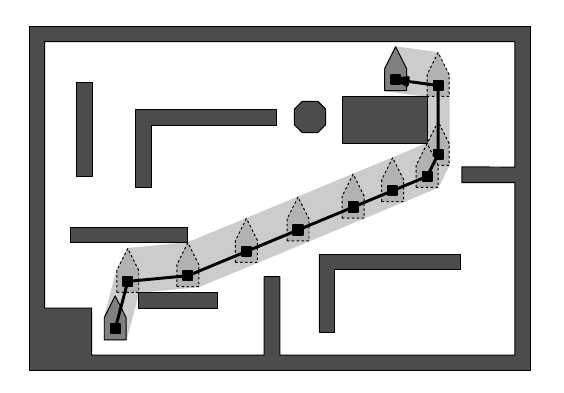
\includegraphics[width=0.60\linewidth]{images/short_path.png}}
% \captionsetup{font=footnotesize}
% \caption{Representaci\'on gr\'afica del camino m\'as corto dentro de un ambiente con obst\'aculos.}
%\label{f:shortPath}
%\end{figure}

En la geometr\'ia computacional y la planificaci\'on del movimiento del 
robot, un mapa de visibilidad es un mapa de ubicaciones intervisibles, 
generalmente para un conjunto de puntos y obst\'aculos en un plano 
euclideano \cite{wikiVisibilityGraph}. Las caracter\'isticas que definen 
un mapa de visibilidad son sus nodos que comparten un borde si se encuentran 
a la vista el uno del otro, y que todos los puntos en el espacio libre del 
robot se encuentren dentro de la l\'inea de visi\'on de al menos un nodo 
en el mapa de visibilidad. 

El gr\'afico de visibilidad est\'andar se define en un espacio de 
configuraci\'on poligonal bidimensional (Figura \ref{f:mapPolygonal}). Los 
nodos $v_{i}$ del gr\'afico de visibilidad incluyen la ubicaci\'on de 
inicio, la ubicaci\'on del objetivo y todos los v\'ertices de los obst\'aculos 
del espacio de configuraci\'on. Los bordes del gr\'afico $e_{ij}$ son 
segmentos de l\'inea recta que conectan dos nodos de l\'inea de vista $v_{i}$ 
y $v_{j}$.

\begin{figure}%[h]
\centering \footnotesize
 {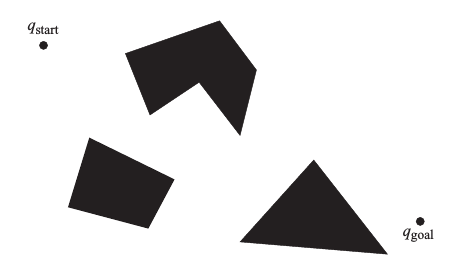
\includegraphics[width=0.60\linewidth]{images/map_polygonal.png}}
 \captionsetup{font=footnotesize}
 \caption{Espacio de configuraci\'on con un punto de inicio y otro punto 
 de llegada a la posici\'on deseada.}
\label{f:mapPolygonal}
\end{figure}

\begin{figure}%[h]
\centering \footnotesize
 {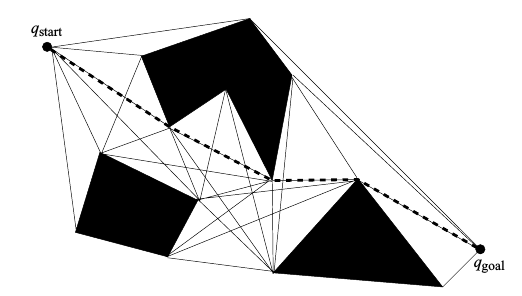
\includegraphics[width=0.60\linewidth]{images/shortPath_visibilityGraph.png}}
 \captionsetup{font=footnotesize}
 \caption{Los obst\'aculos son representado por s\'olidos pol\'igonos. Las 
 l\'ineas continuas delinean los bordes de la visibilidad gr\'afica para 
 los tres obst\'aculos y las l\'ineas entrecortadas representan el camino 
 m\'as corto entre el punto de inicio y el punto de meta.}
\label{f:shortVG}
\end{figure}

A partir de la figura \ref{f:mapPolygonal} se considera la inclusi\'on de 
los nodos y bordes en el espacio libre y que los bordes de los obst\'aculos 
poligonales tambi\'en sirven como bordes en el gr\'afico de 
visibilidad. Utilizando distancia euclidiana se puede buscar la ruta m\'as 
corta como se aprecia en la figura \ref{f:shortVG}.

\subsection{Movimiento Basado en Muestreo Aleatorio}

Las planificaci\'on de movimientos basados en muestreo, como los m\'etodos 
de mapa de ruta probabil\'ista (\textit{Probabilistic Roadmap}) o aquellos 
basados en los \'arboles aleatorios de exploraci\'on r\'apida 
(\textit{Rapidly Exploring Random Trees}) est\'an dando buenos resultados 
en la planificaci\'on de movimientos de robots con muchos grados de 
libertad. Con estos enfoques, se han propuesto varias estrategias para 
predisponer el muestreo hacia las regiones m\'as prometedoras, mejorando 
con esto la eficiencia y permitiendo la soluci\'on de problemas dif\'iciles 
de planificaci\'on de movimientos \cite{elbanhawi2014sampling}. El \'exito 
de estos planificadores en la soluci\'on de problemas desafiantes se puede 
explicar por el hecho de que no se requiere ninguna representaci\'on 
expl\'icita del espacio de configuraci\'on libre. En esta secci\'on se 
explicar\'a los m\'etodos \textit{Probabilistic Roadmap} y \textit{Rapidly 
Exploring Random Trees}.

%\subsubsection{Mapa de Ruta Probabil\'istico (\textit{Probabilistic Roadmap})}
\paragraph{Mapa de Ruta Probabil\'istico (\textit{Probabilistic Roadmap})}

La planificaci\'on del mapa de ruta probabil\'istico (PRM) es una de las 
alternativas para la planificaci\'on de las rutas frente a los  
obst\'aculos, donde las posiciones no se conocen con certeza. El PRM es una 
t\'ecnica popular para la planificaci\'on de caminos en espacios de alta 
dimensi\'on \cite{guibas1999probabilistic}. Este algoritmo es aplicable 
en muchas situaciones, incluida la planificaci\'on del movimiento del 
robot y la planificaci\'on de las rutas de las personas. Las PRM generan 
un gr\'afico aleatorio con v\'ertices que representan las posiciones del 
robot y los bordes representan el movimiento desde una posici\'on a otra 
posici\'on. Seguido a esto se busca,en este gr\'afico, una ruta desde el 
punto de inicio hacia el objetivo. El \'exito de este algoritmo se debe 
a que reducen la b\'usqueda de gr\'aficos. Sin embargo, la mayor\'ia de 
los enfoques de PRM se basan en la suposici\'on de que el planificador 
conoce las ubicaciones de todos los obst\'aculos en el entorno antes de 
construir el gr\'afico del \textit{roadmap} o trazar una ruta. El enfoque 
de este trabajo es que el robot inicialmente no sabe donde est\'an 
ubicados los obst\'aculos.

El algoritmo comienza con muestrear valores aleatorios para cada grado de 
libertad del robot para s\'i poder crear una configuraci\'on completa 
(posici\'on), el planificador de PRM es capaz de \textit{explorar} todo 
el espacio de configuraci\'on (espacio $C$). No todas las configuraciones 
en el espacio ser\'an utilizables debido a obst\'aculos o auto-colisiones, 
por lo que el espacio n-dimensional se divide conceptualmente en dos \'areas 
no contiguas llamadas $C_{free}$ y $C_{obst}$ para configuraciones libres y 
obstruidas, respectivamente. En la fase de preprocesamiento se empieza a 
contruir un gr\'afico PRM usando el algoritmo de muestreo que genera 
aleatoramiente configuraciones para el robot y luego valida las 
posiciones generadas. Lo m\'as simple y com\'un que se hace es rechazar 
todas las posiciones que se cruzan con $C_{obst}$. 

%El gr\'afico se completa tomando cada v\'ertice muestreado e intentando 
%crear $n$ bordes a los v\'ertices vecinos verificando si se encuentra una 
%ruta libre de colisiones entre los dos v\'ertices. En la fase de consulta 
%de PRM, un gr\'afico completado se puede buscar r\'apidamente para las 
%rutas entre dos posiciones arbitrarias utilizando algoritmos de 
%b\'usqueda de gr\'aficos est\'andar.

%Para modelar los obst\'aculos inciertos se asume que se tiene distribuciones 
%de probabilidad sobre las posiciones de los v\'ertices de los obst\'aculo. Se 
%genera un gr\'afico PRM por adelantado en el que algunos bordes pueden 
%intersectar los obst\'aculos inciertos. Luego se construye un plan de 
%ruta que atraviesa el gr\'afico de manera \'optima, dado el hecho de 
%que las observaciones se realizar\'an a medida que el robot se va acercando a 
%los obst\'aculos que permitir\'a determinar qu\'e bordes est\'an 
%libres de obst\'aculos.

%\subsubsection{\'Arbol Aleatorio de Exploraci\'on R\'apida (\textit{Rapidly Exploring Random Trees})}
\paragraph{\'Arbol Aleatorio de Exploraci\'on R\'apida (\textit{Rapidly Exploring Random Trees})}

Un \'arbol aleatorio de exploraci\'on r\'apida (RRT) es un algoritmo que esta dise\~nado para 
buscar de manera eficiente espacios no convexos de gran dimensi\'on. Los RRT se construyen de 
forma incremental de una manera que reduce r\'apidamente la distancia esperada de un punto elegido 
al azar. Los RRT son particularmente adecuados para problemas de planificaci\'on de ruta que 
involucran obst\'aculos y restricciones diferenciales (no holon\'omicas o kinodin\'amicas).

Un RRT hace crecer un \'arbol enraizado en la configuraci\'on inicial utilizando muestras aleatorias 
del espacio de b\'usqueda. A medida que se extrae cada muestra, se intenta establecer una conexi\'on 
entre ella y el estado m\'as cercano en el \'arbol. Si la conexi\'on es factible (pasa completamente 
a trav\'es del espacio libre y obedece a cualquier restricci\'on), esto resulta en la adici\'on del 
nuevo estado al \'arbol. Con un muestreo uniforme del espacio de b\'usqueda, la probabilidad de expandir 
un estado existente es proporcional al tama\~no de su regi\'on de Voronoi. Como las regiones m\'as 
grandes de Voronoi pertenecen a los estados en la frontera de la b\'usqueda, esto significa que el 
\'arbol se expande preferentemente hacia grandes \'areas no buscadas. 

%\subsubsection{Movimiento basado en Mapa de Red (\textit{GridMap})}
\paragraph{Movimiento basado en Mapa de Red (\textit{GridMap})}

La navegaci\'on basada en mapas de red es bastante natural para las personas porque usar un mapa es 
la forma m\'as conveniente de describir un entorno. Sin embargo, el uso de los mapas requiere de 
un buen proceso cognitivo para poder interpretar el mapa y establecer la correspondencia con el 
mundo real.

Para la navegaci\'on basada en mapas de red se pueden usar dos fuentes de informaci\'on. El primero 
es la fuente idiot\'etica, que proporciona informaci\'on interna sobre el movimiento del robot. El 
segundo es la fuente alot\'etica, que proporciona informaci\'on externa sobre el ambiente. La 
informaci\'on idiot\'etica se refiere a la odometr\'ia del robot y la informaci\'on alot\'etica 
se refiere a alg\'un sensor externo que permita al robot tener una perspectiva del entorno donde 
se encuentra.

Dadas las fuentes de informaci\'on como la odometr\'ia y la de un sensor externo, hay muchas formas 
de poder integrarlas en una representaci\'on \'util para la navegaci\'on de los robots. Los 
modelos correspondientes se separan en dos categor\'ias recurriendo a mapas m\'etricos, las posiciones 
de algunos objetos, principalmente los obst\'aculos que el robot puede encontrar, se almacenan en un 
marco de referencia com\'un.

La exploraci\'on con estos mapas de red consiste en que el robot empieza en un punto preparado para 
poder tomar cualquier ruta y realizar varios viajes. Entonces el robot empieza a recibir tareas 
de un nodo central para que pueda desplazarse en diferentes puntos del mapa. El mapa se categoriza 
en tres tipos diferentes: \textit{un obst\'aculo} (probabilidad de ocupaci\'on por encima de un umbral), 
\textit{limpio} (probabilidad de ocupaci\'on nulo) y \textit{desconocido} (nunca se detect\'o nada). De 
esta forma se empieza a construir el mapa y cuando el robot recibe este mapa que se actualiza 
constantemente, empieza a tener una mejor percepci\'on del ambiente donde se encuentra.


\section{Localizaci\'on}
La navegaci\'on es una de las tareas con mayor exigencia para un robot 
m\'ovil. Para realizar una buena navegaci\'on se necesita de cuatro 
componentes b\'asicos los cuales son: (1) percepci\'on, el robot debe extraer 
e interpretar los datos de sus sensores para estimar su entorno; (2) localizaci\'on, 
el robot debe determinar su posici\'on en el entorno; 
(3) cognici\'on, el robot debe tener la capacidad de decidir c\'omo 
actuar para lograr su objetivo; y (4) control de movimiento, el 
robot debe modular sus velocidades para lograr una trayectoria deseada. De los cuatro 
componentes descritos, la localizaci\'on ha recibido la mayor atenci\'on 
de investigaci\'on en la \'ultima d\'ecada y, como resultado, se han logrado
avances significativos. %En esta secci\'on se explicar\'a sobre las metodolog\'ias 
%de localizaci\'on.

El problema en la localizaci\'on es estimar la posici\'on del robot en 
relaci\'on con el mapa del entorno. Cuando un robot se mueve en un entorno 
conocido y comienza en una ubicaci\'on conocida, se puede estimar su posici\'on 
local por medio de la odometr\'ia. Pero esta estimaci\'on de la posici\'on del robot
con el tiempo comienza a volverse menos confiable debido a las incertidumbre,
por ende el robot no tiene una posici\'on absoluta establecida. Con el fin de reducir 
la incertidumbre, el robot tiene que recuperar su posici\'on absoluta localiz\'andose 
en relaci\'on con el mapa. Para ello, el robot debe tener sensores que le permitan 
hacer observaciones del entorno y relacionar estas observaciones con un mapa 
del mundo real. En esta secci\'on se explicar\'a sobre las metodolog\'ias 
de localizaci\'on.

\subsection{Modelo de movimiento y medici\'on}

Un modelo de movimiento probabil\'istico define la transici\'on de la posici\'on 
en dos etapas de tiempo consecutivas ($t-1$ y $t$), despu\'es de que se ha llevado 
a cabo una acci\'on de control ($u_{t}$). Existen dos modelos de movimiento 
probabil\'istico complementarios que son el modelo de movimiento de velocidad y 
el modelo de movimiento de la odometr\'ia. El modelo de movimiento de velocidad 
asume que un robot es controlado a trav\'es de dos velocidades que son la 
velocidad lineal ($v_{t}$) y la velocidad angular ($\omega_{t}$).

\begin{equation}
\label{eqn:modelMotion}
u_{t} = \begin{pmatrix}
v_{t} \\
\omega_{t}
\end{pmatrix}
\end{equation}

Un modelo probabil\'istico de medici\'on describe la relaci\'on entre la posici\'on del 
mundo real y la lectura del sensor (\textit{observaci\'on}). Bas\'andose en la 
estimaci\'on de la posici\'on del mundo real, se genera un \textit{belief} sobre las 
posibles mediciones. Un \textit{belief} es el conocimiento del robot sobre el entorno. El 
ruido en las mediciones del sensor se modela expl\'icitamente, inherente a la incertidumbre 
de los sensores del robot. Para expresae el proceso de generaci\'on de mediciones, se requiere 
una especificaci\'on del entorno. Un mapa ($m$) del entorno es una lista de objetos y ubicaciones:
\begin{align}
m =\{m_{1}, m_{2}, \ldots, m_{N}\}
\end{align}
donde $N$ es el total de n\'umeros de objetos en el ambiente. Los mapas suelen ser mapas 
basados en caracter\'isticas o mapas basados en la ubicaci\'on. Los mapas basados en 
ubicación son volumétricos y ofrecen una etiqueta para cualquier ubicación y los mapas basados 
en características son más populares debido a que la representación hace más fácil ajustar la 
posición de los objetos.

\subsection{Filtros de Kalman}
El filtro de Kalman se basa en la suposición de que el sistema es lineal y tanto el modelo de 
movimiento como el modelo de medición se ven afectados por el ruido gaussiano. El \textit{belief} 
en el tiempo $t$ está representada por una distribución gaussiana multivariable definida por 
su media ($\mu_{t}$) y la covarianza ($\Sigma_{t}$).

Un modelo de transici\'on de estado es definido como:
\begin{align}
\label{eqn:transicion_estado}
p(x_{t}\mid x_{0:t-1}, z_{1:t-1}, u_{1:t}) = p(x_{t}\mid x_{t-1}, u_{t})
\end{align}
donde $p(x_{t}\mid x_{t-1}, u_{t})$ es llamada probabilidad de transición de estado y 
especifica cómo evoluciona el estado del entorno a lo largo del tiempo en función del 
control del robot $u_{t}$.

Un modelo de medici\'on del sensor es definido como:
\begin{align}
\label{eqn:modelo_medicion}
p(z_{t}\mid x_{0:t}, z_{1:t-1}, u_{1:t}) = p (z_{t}\mid x_{t})
\end{align}
donde $p(z_{t}\mid x_{t})$ is llamado probabilidad de medición y especifica cómo se generan 
las mediciones a partir del estado del ambiente $x_{t}$.

El filtro de Kalman asume que el sistema es lineal: la transición de estado 
$A$ (\ref{eqn:transicion_estado}), el modelo de movimiento $B$ (\ref{eqn:modelMotion})  
y el modelo del sensor $C$ (\ref{eqn:modelo_medicion}) son funciones lineales únicamente 
dependiendo del estado $x$ o del comando de control ($u$), más un modelo 
de ruido gaussiano ($Q$):
\begin{equation*}
\label{eqn: Kalman Filter}
\begin{matrix}
\textrm{\textbf{Predicción}}\\
\overline{\mu}_{t} &= &A_{t}\mu_{t-1} + B_{t} u_{t} &\textrm{estimación de la media a-priori}\\
\overline{\Sigma}_{t} &= &A_{t}\Sigma_{t-1} A_{t}^{T} + R_{t} &\textrm{estimación de la covarianza a-priori}\\
\textrm{\textbf{Actualización}}\\
K_{t} &= &\overline{\Sigma}_{t}C_{t}^{T}(C_{t}\overline{\Sigma}_{t}C_{t}^{T} + Q_{t})^{-1} &\textrm{Ganancia de Kalman}\\
\mu_{t} &= &\overline{\mu}_{t} + K_{t}(z_{t} - C_{t}\overline{\mu}_{t}) &\textrm{actualización estimación de estado (a posteriori)}\\
\Sigma_{t} &= &(I - K_{t}C_{t})\overline{\Sigma}_{t} &\textrm{actualización estimación de la covarianza (a posteriori)}\\
\end{matrix}
\end{equation*}

Cuando se realiza una medici\'onn, se hace una predicci\'on de un \textit{belief} 
($bel(x_{t})$),\\ basado en el \textit{belief} anterior $bel(x_{t-1})$, tambi\'en de los 
datos de control ($u_{t}$) y del modelo de transición de estado. Este nuevo \textit{belief}
describe el estado más probable ($\overline{\mu}_{t}$) en el tiempo ($t$) y la covarianza 
($\overline{\Sigma}_{t}$). En la etapa de la actualización, el \textit{belief} que fue predecido 
cambia, incorporando la medici\'on ($z_{t}$). La ganancia de Kalman ($K_{t}$) especifica el
grado que la medici\'on se incorpora en la nueva estimación del estado. El concepto principal 
del filtro de kalman es la innovaci\'on, que significa la diferencia entre la medici\'on 
real y la medici\'on esperada ($C_{t}\overline{\mu}_{t}$), que se deriva del estado que fue 
predecido. Una medida que está lejos de la medida predecida, es menos confiable, por lo tanto 
es menos probable que se incorpore en la nueva estimación del estado.

El filtro de Kalman estándar requiere un sistema lineal, que no es suficiente para 
describir muchos problemas de la vida real. Por lo tanto, se han propuesto 
variaciones del algoritmo original que pueden hacer frente a diferentes niveles de 
no-linealidad. Estas variaciones se aproximan a los modelos de movimiento y medición 
de forma que tiendan a ser lineales.


\subsection{Filtros de Part\'iculas}
El filtro de part\'iculas es una implementaci\'on alternativa no param\'etrica, al igual 
que los filtros de histograma, los filtros de part\'iculas se aproximan al estado posterior 
por un n\'umero finito de par\'ametros. Sin embargo, difieren en la forma en que se generan 
estos par\'ametros, y en los que muestrean el espacio de estado. La idea del filtro de 
part\'iculas es representar el \textit{belief} predecido ($x_{t}$), mediante un conjunto de 
muestras aleatorias de estado. En lugar de representar la distribuci\'on mediante una forma 
param\'etrica (la funci\'on exponencial que define la densidad de una distribuci\'on normal), 
los filtros de part\'iculas representan una distribuci\'on por un conjunto de muestras extra\'idas 
de esta distribuci\'on. Tal representaci\'on es aproximada, pero no es param\'etrica, por 
lo tanto se puede representar un espacio de distribuciones mucho m\'as amplio que los gaussianos.


\subsection{Filtros de Informaci\'on}
El filtro de informaci\'on (IF) representa el \textit{belief} por medio de un gaussiano. Por lo 
tanto, el filtro de informaci\'on est\'andar est\'a sujeto a las mismas suposiciones subyacentes 
al filtro de Kalman (KF). La diferencia entre el KF y el IF surge de la forma que se representa 
el \textit{belief} gaussiano. Mientras que en la familia de algoritmos de filtro de Kalman, los 
gaussianos est\'an representados por sus momentos (media, covarianza), en cambio los filtros de 
informaci\'on representan gaussianos en su representaci\'on can\'onica, que est\'a compuesta por 
una matriz de informaci\'on y un vector de informaci\'on. La diferencia en la representaci\'on 
conduce a diferentes ecuaciones de actualizaci\'on. En particular, lo que es computacionalmente 
complejo en una representaci\'on resulta ser simple en la otra y viceversa. Las representaciones 
can\'onicas y de momentos a menudo se consideran duales entre s\'i, y as\'i son el IF y el KF.

\section{Mapeo y Localizaci\'on Simult\'anea (\textit{SLAM})}
Un problema mucho m\'as dif\'icil de la localizaci\'on es cuando no conoces el mapa del ambiente. En 
este caso, la informaci\'on del sensor del robot se utiliza para recuperar la trayectoria del robot 
y construir un mapa del entorno. Este problema se llama mapeo y localizaci\'on simult\'anea 
(\textit{SLAM}). Una soluci\'on a este problema har\'ia que un robot sea totalmente 
aut\'onomo. \textit{SLAM} es un problema dif\'icil porque tanto el camino estimado como el mapa 
construido son afectados por el ruido. Ambos se vuelven cada vez m\'as inexactos durante el viaje. Sin 
embargo, cuando se revisa un lugar que ha sido mapeado, se puede reducir la incertidumbre. Este proceso 
se denomina cierre de bucle. Adem\'as, se puede optimizar el mapa despu\'es de que se detecta un evento 
de cierre de bucle. En esta secci\'on se explicar\'a los m\'etodos de \textit{SLAM} m\'as utilizados 
actualmente.

\subsection{EKF SLAM}
El \textit{SLAM} basado en el filtro extendido de kalman es el algoritmo m\'as antiguo y el m\'as influyente. El
algoritmo \textit{EKF-SLAM} aplica el \textit{EKF} al \textit{SLAM} usando la asociaci\'on de datos de m\'axima 
verosimilitud. Al hacerlo, \textit{EKF-SLAM} est\'a sujeto a una serie de aproximaciones y suposiciones
limitantes:
\begin{itemize}
	\item[•] \textit{\textbf{Mapas basados en funciones:}} Los mapas, en el \textit{EKF}, se componen de puntos
	de referencia. Por razones de computaci\'on, el n\'umero de puntos de referencia es generalmente
	peque\~no (por ejemplo, m\'as peque\~no que 1000). Adem\'as, el enfoque de \textit{EKF} tiende a
	funcionar bien cuanto menos ambiguos son los hitos. Por esta raz\'on, \textit{EKF-SLAM} requiere una
	ingenier\'ia significativa de los detectores de funciones, a veces utilizando balizas
	artificiales o puntos de referencia como caracter\'isticas.
	\item[•] \textit{\textbf{Ruido Gaussiano:}} Como cualquier algoritmo \textit{EKF}, \textit{EKF-SLAM} 
	hace una suposici\'on de ruido Gaussiano para el movimiento del robot y la percepci\'on. La
	cantidad de incertidumbre en la parte de la predicci\'on debe ser relativamente
	peque\~na, ya que de lo contrario la linealizaci\'on en \textit{EKF} tiende a introducir 
	errores intolerables.
	\item[•] \textit{\textbf{Mediciones positivas:}} El algoritmo \textit{EKF-SLAM}, al igual 
	que el localizador \textit{EKF}, solo puede procesar avistamientos positivos de hitos. No
	puede procesar informaci\'on negativa que surge de la ausencia de puntos de referencia en 
	las mediciones de un sensor. Esta es una consecuencia directa de la representaci\'on
	de \textit{belief} gaussiano.
\end{itemize}

\subsection{FastSLAM}
FastSLAM descompone el problema SLAM en un problema de localizaci\'on de robot, y una colecci\'on 
de problemas de estimaci\'on de puntos de referencia (\textit{landmarks}) que est\'an condicionados 
a la estimaci\'on de la posici\'on del robot. Como se se\~nala en \cite{murphy2000bayesian}, esta 
representaci\'on factorizada es exacta, debido a las independencias condicionales naturales en el 
problema SLAM. FastSLAM usa un filtro de part\'iculas modificado para estimar el camino predecido 
sobre el robot. Cada part\'icula posee filtros de Kalman que estiman las ubicaciones de los puntos 
de referencia condicionadas en la estimaci\'on de la ruta. La implementaci\'on de este algoritmo 
requiere tiempo.

\subsection{GraphSLAM}
SLAM basado en gr\'aficos construye un problema de estimaci\'on simplificado al extraer las mediciones 
del sensor sin ser procesadas. Estas medidas se reemplazan por los bordes en el gr\'afico que luego 
se pueden ver como "medidas virtuales". M\'as detalladamente, un borde entre dos nodos se etiqueta 
con una distribuci\'on de probabilidad sobre las ubicaciones relativas de las dos posturas, 
condicionadas a sus mediciones mutuas. En general, el modelo de observaci\'on $p(z_{t}| x_{t},  
m_{t})$ es multimodal y, por lo tanto, el supuesto gaussiano no se cumple. Esto significa que una 
\'unica observaci\'on $z_{t}$ puede dar como resultado m\'ultiples aristas potenciales que 
conectan diferentes posiciones en el gr\'afico y la conectividad del gr\'afico necesita ser descrita 
como una distribuci\'on de probabilidad. 
Dirigirse directamente a esta multimodalidad en el proceso de estimaci\'on llevar\'ia a una explosi\'on combinatoria de la complejidad. Como resultado de eso, la mayor\'ia de los enfoques pr\'acticos restringen 
la estimaci\'on a la topolog\'ia m\'as probable. Por lo tanto, se necesita determinar la restricci\'on 
m\'as probable resultante de una observaci\'on. Esta decisi\'on depende de la distribuci\'on de 
probabilidad sobre las posiciones del robot.

%\section{Robótica Probabilística}

%Para el desarrollo de esta tesis se utilizó como herramienta los fundamentos de la  Robótica Probabilística, esta basado en el libro de Sebastian Thrun \cite{Thrun2005}.Para que el robot pueda saber sobre el ambiente donde se encuentra, necesita utilizar sensores.Los sensores tienen una limitación en lo que pueden percibir (por ejemplo, el alcance y la resolución). Estos también están sujetos a ruido, lo que desvía las mediciones de los sensores de maneras impredecibles. Este ruido limita la información que se puede extraer de las mediciones del sensor. Los actuadores del robot (por ejemplo,motores) también están sujetos a ruido, lo que introduce incertidumbre. Otra fuente de incertidumbre es causada por el software del robot, que utiliza modelos aproximados del mundo real. Los errores de modelo son una fuente de incertidumbre que a menudo se ha ignorado en los robots. Los robots son sistemas en tiempo real y esto requiere el uso de aproximaciones algorítmicas, pero aumenta la cantidad de incertidumbre aún más.

%Para algunas aplicaciones robóticas (por ejemplo, robots KUKA utilizado en industrias), la incertidumbre es un factor marginal. Dado que los robots están cada vez más desplegados en el mundo abierto, la cuestión de la incertidumbre se ha convertido en un gran desafío para el diseño de robots capaces. La robótica probabilística es un enfoque relativamente nuevo de la robótica que presta atención a la incertidumbre en la percepción y la acción. La incertidumbre se representa explícitamente usando el cálculo de la teoría de la probabilidad. Esto significa que los algoritmos probabilísticos representan la información por distribuciones de probabilidad sobre un espacio. Esto permite representar la ambigüedad y el grado de creencia de una manera matemáticamente correcta. Ahora, los robots pueden tomar decisiones con respecto a la incertidumbre que permanece, o eligieron reducir la incertidumbre si esa es la mejor opción (para esta tesis, exploración).


%\subsection{Estimación del estado recursivo}

%\textbf{Definición 1.} Los ambientes se caracterizan por el estado, que describe todos los aspectos de un robot y el medio ambiente que pueden afectar el futuro. Un estado puede ser un \textit{estado estático}(no cambiante) o un \textit{estado dinámico} (cambiante) en el que ciertas variables de estado tienden a cambiar con el tiempo. Un estado se denomina $x$. El estado en el tiempo $t$ se denota $x_{t}$.

%Las variables del estado son:
%\begin{itemize}
%\item[•] \textit{La pose del robot}: Es la localización y orientación del robot con respecto a un marco global de coordenadas.
%\item[•] \textit{La velocidad del robot}: Es la velocidad para cada pose del robot.
%\item[•] \textit{La ubicación y características de los objetos en el entorno}: Los objetos pueden ser estáticos o dinámicos. Los objetos son modelados como puntos de referencia, cada uno con características distintas y estacionarias que permiten un reconocimiento fiable.
%\end{itemize}

%Una de las ideas de la robótica probabilística es la estimación del estado a partir de los datos del sensor, pero los sensores solo observan una parte de la información total y sus mediciones se ven afectadas por el ruido. Por ende la estimación del estado intenta recuperar las variables de estado a partir de los datos. En lugar de calcular un único estado, este calcula una distribución probabilística sobre los posibles estados en el mundo real.Esta distribución probabilística es llamada \textit{belief} y es descrita en la siguiente página.

%\textbf{Definición 2.} La estimación de estados se encargan del problema de estimar las varibales de estado a partir de los datos de los sensores que no son directamente observables, pero se puede inferir. Una distribución probabilística se calcula sobre los posibles estados del mundo real.

%Un robot puede interactuar con su entorno influyendo en el estado de su entorno a través de sus actuadores (acciones de control), o puede recopilar información sobre el estado a través de sus sensores (mediciones del sensor en el ambiente).

%\textbf{Definición 3.} El conjunto de todas las mediciones adquiridas desde el tiempo $t_{1}$ hasta el tiempo $t_{2}$, para $t_{1} \leqslant t_{2}$ es igual a:
%\begin{equation}
%z_{t_{1}:t_{2}} = z_{t_{1}}, z_{t_{1} + 1}, z_{t_{1} + 2}, \ldots , z_{t_{2}}
%\end{equation}
 
%\textbf{Definición 4.} El conjunto de todos los datos de control desde el tiempo $t_{1}$ hasta el tiempo $t_{2}$, para $t_{1} \leqslant t_{2}$ es igual a:
%\begin{equation}
%u_{t_{1}:t_{2}} = u_{t_{1}},u_{t_{1} + 1}, u_{t_{1} + 2}, \ldots , u_{t_{2}}
%\end{equation}

%Los datos de control transmiten información relativa al cambio de estado. Por ejemplo, establecer la velocidad de un robot a 1 $m/s$, sugiere que la nueva posición del robot después de 2 segundos está aproximadamente 2 metros por delante de su posición antes de ejecutar el comando.
%Generalmente, las mediciones proporcionan información sobre el estado del ambiente, aumentando el conocimiento del robot. El problema de esta información es que el movimiento del robot tiende a inducir una pérdida de conocimiento debido al ruido inherente en el accionamiento del robot.
%La evolución del estado y las mediciones se realizan mediante leyes probabilísticas.El estado ~$x_{t}$ es generado estocásticamente desde el estado ~$x_{t-1}$. Cuando se dice que el estado ~$x_{t}$ es completo, implica que se sabe ~$x_{t-1}$.Las mediciones pasadas y los controles no transmiten ninguna información con respecto al estado ~$x_{t}$. Esta suposición se conoce como \textit{Markov Assumption} y se expresa de la siguiente forma:
%\begin{equation}
%\label{eqn:markov-assumption1}
%p(x_{t}\mid x_{0:t-1}, z_{1:t-1}, u_{1:t}) = p(x_{t}\mid x_{t-1}, u_{t})
%\end{equation}
%donde $p(x_{t}\mid x_{t-1}, u_{t})$ es llamada probabilidad de transición de estado y especifica cómo evoluciona el estado ambiental a lo largo del tiempo en función del control del robot $u_{t}$.  

%\textbf{Definición 5.} \textit{Markov Assumption} establece que los datos pasados y futuros son independientes si se conoce el estado actual $x_{t}$. Esto significa que los valores en cualquier estado son influenciados solamente por los valores del estado que lo precedieron directamente.
%El proceso por el cual se modelan las mediciones se expresa:
%\begin{equation}
%\label{eqn:markov-assumption2}
%p(z_{t}\mid x_{0:t}, z_{1:t-1}, u_{1:t}) = p (z_{t}\mid x_{t})
%\end{equation}
%donde $p(z_{t}\mid x_{t})$ is llamado probabilidad de medición y especifica cómo se generan las mediciones a partir del estado del ambiente $x_{t}$.

%Otra idea de la robótica probabilística es \textit{belief}, que refleja el conocimiento del robot sobre el estado del mundo real. Las distribuciones de creencias son probabilidades posteriores sobre variables de estado condicionadas a los datos disponibles. \textit{Markov Assumption} implica que la creencia actual es suficiente para representar la historia pasada del robot. El \textit{belief} sobre las variables de estado se expresa como $bel(x_{t})$:
%\begin{equation}
%bel(x_{t}) = p(x_{t}\mid z_{1:t}, u_{1:t})
%\end{equation}

%Se puede realizar una predicción del estado en el tiempo $t$ antes de incorporar una medición. Esta predicción es usada en el contexto del filtrado probabilístico y es denotado como:
%\begin{equation}
%\overline{bel}(x_{t}) = p(x_{t}\mid z_{1:t-1}, u_{1:t})
%\end{equation}
%esta ecuación predice el estado en el tiempo ~$t$ basado en el estado anterior, antes de incorporar la medida en el tiempo ~$t$.

%\textbf{Definición 6.} \textit{Belief} refleja el conocimiento del robot sobre el estado del entorno, a través de distribuciones de probabilidad condicional. \textit{Belief} sobre la variable de estado $x_{t}$ es denotado por $bel(x_{t})$.


%\subsection{Algoritmos}

%El algoritmo más general para calcular los \textit{belief} es el filtro de Bayes. La entrada del algoritmo es el \textit{belief} $bel$ en el instante $t-1$, el control $u_{t}$ más reciente y la medición $z_{t}$. En primer lugar, se calcula una predicción para la nueva creencia basada en el control $u_{t}$ (la medición es ignorada):
%\begin{equation}
%\label{eqn:BF-prediction}
%\overline{bel}(x_{t}) = \int p(x_{t}\mid u_{t},x_{t-1})bel(x_{t-1})dx_{t-1}.
%\end{equation}
%El segundo paso de los filtros de bayes es la medición actualizada:
%\begin{equation}
%\label{eqn:BF-measurement}
%bel(x_{t}) = \eta p(z_{t}\mid x_{t})\overline{bel}(x_{t})
%\end{equation}
%donde $\eta$ es una constante de normalización para asegurar una probabilidad válida. Ahora,$bel(x_{t})$ es el \textit{belief} del robot sobre el estado, después los datos de medición y control se usan para mejorar el conocimiento del robot. Ambos pasos del algoritmo se realizan recursivamente para todas las mediciones y comandos de control.

%La familia más popular de los estimadores de estado recursivos son los filtros gaussianos. Los filtros gaussianos representan el \textit{belief} mediante distribuciones normales multivariadas (aproximadas por una función gaussiana). 
%\begin{equation}
%p(x)= det(2\pi\Sigma)^{-\frac{1}{2}} exp\{-\frac{1}{2}(x-\mu)^{T}\Sigma^{-1}(x-\mu)\}
%\end{equation}
%La función densidad (probabilidad) sobre el espacio de estado $x$ se caracteriza por dos parámetros: la media $\mu$ y la covarianza $\Sigma$.
%Los gaussianos son unimodales y tienen un único máximo. Sin embargo, esto es característico para muchos problemas de seguimiento, donde el posterior se centra alrededor del estado verdadero con un cierto margen de incertidumbre.
%Con el fin de implementar los filtros descritos anteriormente, se requiere dos componentes adicionales. En la sección 2.2.3,se describe el modelo de movimiento y en la sección 2.2.4 se describe el modelo de medición.


%\subsection{Modelo de Movimiento}

%Los modelos de movimiento probabilísticos describen la relación entre la pose anterior con la actual, también lo controles (comandos) emitidos por una distribución de probabilidad. Esto es llamado como la probabilidad de transición de estado. La probabilidad de transición de estado juega un papel esencial en la etapa de predicción del filtro de Bayes.

%\textbf{Definición 7.} Un modelo de movimiento probabilístico define la transición de estado entre dos etapas de tiempo consecutivas $t-1$ y $t$ después de que se ha llevado a cabo una acción de control $u_{t}$. Se expresa por la distribución posterior $p(x_{t}\mid x_{t-1}, u_{t})$.

%Existe dos modelos de movimiento probabilístico complementarios que son el modelo de movimiento de velocidad y el modelo de movimiento de odometría. El modelo de movimiento de velocidad asume que un robot es controlado a través de dos velocidades: una velocidad de rotación $\omega_{t}$ y la velocidad de traslación $v_{t}$.
%\begin{equation}
%u_{t} = \begin{pmatrix}
%v_{t} \\
%\omega_{t}
%\end{pmatrix}
%\end{equation}

%La probabilidad $p(x_{t}\mid x_{t-1}, u_{t})$ se puede calcular con algoritmos que se pueden encontrar en \cite{Thrun2005}. El modelo de movimiento de odometría asume que uno tiene acceso a la información de los encoders de la rueda. En la práctica, los modelos de odometría tienden a ser más precisos, porque la mayoría de los robots no ejecutan el comando de velocidad con el nivel de precisión que se obtiene midiendo la odometría. Técnicamente, las lecturas de odometría no son controles porque se reciben después de ejecutar un comando. Sin embargo, el uso de lecturas de odometría como controles da como resultado una formulación más sencilla del problema de estimación.

%Ambos modelos no se pueden aplicar a los drones. Por ejemplo, un quadcopter es controlado a través de sus ángulos de rotación (pitch, roll y yaw). Se requiere una conversión entre ángulos y velocidades para usar el modelo de movimiento de velocidad para un quadcopter. Para los robots de tierra, la odometría puede obtenerse mediante la integración de la lectura de los encoders de cada rueda, pero un quadcopter no tiene contacto con el suelo, por ende no se puede realizar odometría. En su lugar, se utilizan diferentes fuentes de información para obtener información de odometría. Por ejemplo, el quadcopter de esta tesis utilizará un sensor láser para obtener esta información.

%\subsection{Modelo de Medición}

%Los modelos probabilísticos de medición describen la relación entre los estados del mundo real $x_{t}$ y cómo se realiza un lectura del sensor $z_{t}$ (observación). Basándose en el estado estimado del mundo real $x_{t}$, se genera un \textit{belief} sobre las posibles mediciones. El ruido en las mediciones del sensor se modela explícitamente, inherente a la incertidumbre de los sensores del robot. Para expresar el proceso de generación de mediciones, se requiere una especificación del entorno. Un mapa $m$ del entorno es una lista de objetos y ubicaciones:
%\begin{equation}
%m =\{m_{1}, m_{2}, \ldots, m_{N}\}
%\end{equation}
%donde $N$ es el total de números de objetos en el ambiente.Los mapas suelen ser mapas basados en características o mapas basados en la ubicación. Los mapas basados en ubicación son volumétricos y ofrecen una etiqueta para cualquier ubicación. Los mapas basados en funciones sólo describen la forma del entorno en ubicaciones específicas, que son comúnmente objetos. Los mapas basados en características son más populares debido a que la representación hace más fácil ajustar la posición de los objetos.

%\textbf{Definición 8.} Un modelo de sensor probabilístico describe la relación entre un estado del mundo real $x_{t}$ y la lectura del sensor $z_{t}$ dado un modelo del ambiente $m$ en forma de una distribución posterior $p(z_{t}\mid x_{t},m)$.

%\subsection{Localización}
%El problema de la localización de un robot es estimar la posición (estado) del robot en relación con el mapa del entorno. La localización es un componente importante para la navegación de un robot, junto con la percepción, la cognición y el control de movimiento.

%Cuando un robot se mueve en un entorno conocido y comienza en una ubicación conocida, puede realizar un seguimiento de su ubicación mediante la integración de estimaciones de posición local (por ejemplo, odometría). Debido a la incertidumbre de estas estimaciones locales, la incertidumbre de la ubicación absoluta del robot aumenta con el tiempo. Con el fin de reducir la incertidumbre, el robot tiene que recuperar su posición absoluta localizándose en relación con un mapa. Para ello, el robot utiliza sus sensores para hacer observaciones de su entorno y relaciona estas observaciones con un mapa del medio ambiente.

%Un enfoque probabilístico de la localización utiliza el \textit{belief} para representar la localización global estimada. De nuevo, actualizar la posición del robot implica dos pasos. El primer paso se denomina actualización de predicción. El robot utiliza su estado en el tiempo $t-1$ y los datos del control $u_{t}$ para predecir su estado en el instante $t$. Este paso de predicción aumenta la incertidumbre sobre el estado del robot. El segundo paso se llama actualización de la percepción. En este paso, el robot utiliza la información de sus sensores para corregir la posición estimada durante la fase de predicción, reduciendo la incertidumbre sobre el estado del robot.

%\subsection{Mapeo y Localización simultánea (SLAM)}
%Un problema mucho más difícil de la localización es cuando no conoces el mapa del ambiente. En este caso, la información del sensor del robot se utiliza para recuperar la trayectoria del robot y construir un mapa del entorno.
%Este problema se llama Mapeo y Localización simultánea (\textit{SLAM}). Una solución a este problema haría  un robot auténticamente autónomo. \textit{SLAM} es un problema difícil porque tanto el camino estimado como el mapa construido son afectados por el ruido. Ambos se vuelven cada vez más inexactos durante el viaje. Sin embargo, cuando se revisa un lugar que ha sido mapeado, se puede reducir la incertidumbre.
%Este proceso se denomina cierre de bucle. Además, se puede optimizar el mapa después de que se detecta un evento de cierre de bucle.
%\subsubsection{Técnicas de Solución}
%En la práctica, no es posible calcular analíticamente el \textit{belief} del robot (probabilidades posteriores). Por lo tanto, existen varias técnicas de aproximación. Esta sección describe las técnicas de solución más populares para los problemas de \textit{SLAM}.

%Las técnicas de solución se pueden dividir en dos ramas principales de la representación del \textit{belief}: \textit{single-hypothesis belief} y \textit{multi-hypothesis belief}. \textbf{Single-hypothesis trackers} representan la creencia de un solo estado del mundo real. Esta estimación esta asociada por una medida de certidumbre (o varianza), que permite al rastreador ampliar o estrechar la región estimada en el espacio de estado. La principal ventaja de la representación \textit{single-hypothesis} es la ausencia de la ambigüedad, simplificando la toma de decisiones en el nivel cognitivo del robot (por ejemplo, la planificación de la trayectoria). Debido a la ausencia de ambigüedad, los rastreadores no modelan adecuadamente las ambigüedades.

%\textbf{Multi-hypothesis trackers} representa el \textit{belief} no solo como un único estado del mundo real, sino como un conjunto posiblemente infinito de estados. La principal ventaja de la representación \textit{multi-hypothesis} es que el robot puede mantener explícitamente la incertidumbre respecto a sus estado. Esto permite a un robot creer en múltiples poses simultáneamente, permitiendo al robot rastrear y rechazar diferentes hipótesis independientemente. Una de las principales desventajas de una representación \textit{multi-hypothesis} implica la toma de decisiones. Si el robot representa su posición como un conjunto de puntos, se vuelve menos obvio calcular la mejor acción.

%Además, las técnicas de solución se pueden dividir en dos ramas de las limitaciones de tiempo: \textit{online computing} y \textit{offline computing}. Las técnicas \textbf{online} resuelven un problema en tiempo real y deben garantizar la respuesta dentro de estrictas restricciones de tiempo. Una ventaja de las técnicas en línea es la capacidad de utilizar la respuesta como entrada para la toma de decisiones (por ejemplo, la navegación), que es esencial para los robots autónomos. Debido a las estrictas restricciones de tiempo, se puede realizar una cantidad limitada de cálculos, lo que limita la complejidad de las técnicas de solución.

%Las técnicas \textbf{offline} tienen restricciones de tiempo menos estrictas, lo que permite una mayor complejidad. Por ejemplo, se pueden realizar mejoras adicionales que serían demasiado lentas para las técnicas en línea. Una de las principales desventajas de las técnicas \textit{offline} implica la toma de decisiones. Debido a que una respuesta no está disponible en tiempo real, el robot tiene que esperar o tomar una decisión sin incorporar la respuesta.

%\textbf{Filtro de Kalman (KF)}

%La técnica más popular para implementar un filtro de Bayes es el Filtro de Kalman (1960) \cite{kalman1960new}, es mayormente utilizado para mejorar la navegación de vehículos. El filtro tiene una representación de \textit{single-hypothesis belief} y se puede realizar en tiempo real. El filtro de Kalman se basa en la suposición de que el sistema es lineal y tanto el modelo de movimiento como el modelo de medición se ven afectados por el ruido gaussiano.El \textit{belief} en el tiempo $t$ está representada por una distribución gaussiana multivariable definida por su media $\mu_{t}$ y la covarianza $\Sigma_{t}$. Esto significa que $x_{t}$ del filtro de Bayes (ecuaciones \ref{eqn:BF-prediction} y \ref{eqn:BF-measurement}) ha sido reemplazado por $\mu_{t}$ y $\Sigma_{t}$.

%El filtro de Kalman asume que el sistema es lineal: la transición de estado $A$ (ecuación \ref{eqn:markov-assumption1}), el modelo de movimiento $B$ y el modelo del sensor $C$ (ecuación \ref{eqn:markov-assumption2}) son funciones lineales únicamente dependiendo del estado $x$ o del comando de control $u$, más un modelo de ruido gaussiano $Q$:
%\begin{equation}
%\label{eqn: Kalman Filter}
%\begin{matrix}
%\textrm{\textbf{Predicción}}\\
%\overline{\mu}_{t} &= &A_{t}\mu_{t-1} + B_{t} u_{t} &\textrm{estimación de la media a-priori}\\
%\overline{\Sigma}_{t} &= &A_{t}\Sigma_{t-1} A_{t}^{T} + R_{t} &\textrm{estimación de la covarianza a-priori}\\
%\textrm{\textbf{Actualización}}\\
%K_{t} &= &\overline{\Sigma}_{t}C_{t}^{T}(C_{t}\overline{\Sigma}_{t}C_{t}^{T} + Q_{t})^{-1} &\textrm{Ganancia de Kalman}\\
%\mu_{t} &= &\overline{\mu}_{t} + K_{t}(z_{t} - C_{t}\overline{\mu}_{t}) &\textrm{actualización estimación de estado (a posteriori)}\\
%\Sigma_{t} &= &(I - K_{t}C_{t})\overline{\Sigma}_{t} &\textrm{actualización estimación de la covarianza (a posteriori)}\\
%\end{matrix}
%\end{equation}

%El filtro de Kalman representa el \textit{belief} $bel(x_{t})$ en el tiempo $t$ por la media $\mu_{t}$ y la covarianza $\Sigma_{t}$. Cuando se recibe una medición, se predice una nueva creencia $bel(x_{t})$ basada en el \textit{belief} anterior $bel(x_{t-1})$, los datos de control $u_{t}$ y tanto el modelo de transición de estado como el modelo de movimiento. Este \textit{belief} predecida describe el estado más probable $\overline{\mu}_{t}$ en el tiempo $t$ y la covarianza $\overline{\Sigma}_{t}$. La medición todavía no está incluida, porque es un \textit{belief} que se predice. El paso de la actualización cambia el \textit{belief} predecido ($\overline{\mu}_{t},\overline{\Sigma}_{t}$) en el \textit{belief} deseado ($\mu_{t},\Sigma_{t}$), incorporando la medición $z_{t}$. La ganancia de Kalman $K_{t}$ especifica el grado que la medición se incorpora en la nueva estimación del estado. El concepto clave utilizado para filtración de kalman es la innovación, que es la diferencia entre la medición real $z_{t}$ y la medición esperada $C_{t}\overline{\mu}_{t}$, que se deriva del estado predecido. Una medida $z_{t}$ que está lejos de la medida predecida, es menos fiable, por lo tanto es menos probable que se incorpore en la nueva estimación del estado.

%El filtro de Kalman estándar requiere un sistema lineal, que no es suficiente para describir muchos problemas de la vida real. Por lo tanto, se han propuesto variaciones del algoritmo original que pueden hacer frente a diferentes niveles de no-linealidad. Estas variaciones se aproximan a los modelos de movimiento y medición de forma que tiendan a ser lineales.

%\textbf{Filtro Extendido de Kalman}

%El filtro extendido de Kalman es una variante del filtro de Kalman que puede utilizarse para sistemas no lineales. Este intenta aproximar los modelos de movimiento y de medición no lineales a sistemas lineales. La probabilidad de transición de estado y las probabilidades de medición son representadas por las funciones no lineales $g$ y $h$:
%\begin{equation}
%\begin{matrix}
%x_{t} &= & g(u_{t},x_{t-1})\\
%z_{t} &= & h(x_{t}) + \delta_{t}
%\end{matrix}
%\end{equation}
%estas funciones reemplazan las matrices de operación A,B y C del filtro de Kalman (ecuación \ref{eqn: Kalman Filter}).

%La idea clave de la aproximación de Filtro Extendido de Kalman se llama linealización. Una aproximación lineal de primer orden de Taylor se calcula a la medida de la creencia actual (Gaussiana), resultando una función lineal. Proyectar la creencia gaussiana a través de la aproximación lineal da como resultado una densidad gaussiana.
%\begin{equation}
%\begin{matrix}
%\textrm{\textbf{Predicción}}\\
%\overline{\mu}_{t} &= &g(u_{t},\mu_{t-1}) &\textrm{estimación de la media a-priori}\\
%\overline{\Sigma}_{t} &= &G_{t}\Sigma_{t-1}G_{t}^T + R_{t} &\textrm{estimación de la covarianza a-priori}\\
%\textrm{\textbf{Actualización}}\\
%K_{t} &= &\overline{\Sigma}_{t}H_{t}^{T}(H_{t}\overline{\Sigma}_{t}H_{t}^{T} + Q_{t})^{-1} &\textrm{Ganancia de Kalman}\\
%\mu_{t} &= &\overline{\mu}_{t} + K_{t}(z_{t} - h(\overline{\mu}_{t})) &\textrm{actualización estimación de estado (a posteriori)}\\
%\Sigma_{t} &= &(I - K_{t}H_{t})\overline{\Sigma}_{t} &\textrm{actualización estimación de la covarianza (a posteriori)}.\\
%\end{matrix}
%\end{equation}

